\documentclass[tikz,border=8pt]{standalone}
% Shared look for every TikZ diagram. Load with \input{../../tools/tikz-style.tex}
\usepackage[T1]{fontenc}
\usepackage{lmodern}
\renewcommand{\sfdefault}{lmr}  % diagrams use the same serif as the text
\usetikzlibrary{arrows.meta, positioning, shapes.geometric, calc, fit, backgrounds}
\definecolor{cblue}{HTML}{4C78A8}
\definecolor{corange}{HTML}{F58518}
\definecolor{cgreen}{HTML}{54A24B}
\definecolor{cred}{HTML}{E45756}
\definecolor{cpurple}{HTML}{B279A2}
\definecolor{cgrey}{HTML}{6B6B6B}
\tikzset{
  every picture/.style={font=\sffamily, line width=1.2pt},
  box/.style={draw=#1, fill=#1!12, rounded corners=4pt, align=center, inner sep=7pt, minimum height=1.1cm},
  box/.default=cgrey,
  arrow/.style={-{Stealth[length=3mm]}, draw=cgrey, line width=1.4pt},
  title/.style={font=\sffamily\bfseries\Large},
  note/.style={font=\sffamily\small, text=cgrey, align=center},
}
\AtBeginDocument{\hyphenpenalty=10000 \exhyphenpenalty=10000}

% A landmark reading: from the robot at (2, 1) facing 30 deg, the pink pole at (1, 3) is at range r = 2.236 m and
% bearing phi = 86.6 deg (measured from the robot's heading, positive to the left); its signature is "pink".
\begin{document}
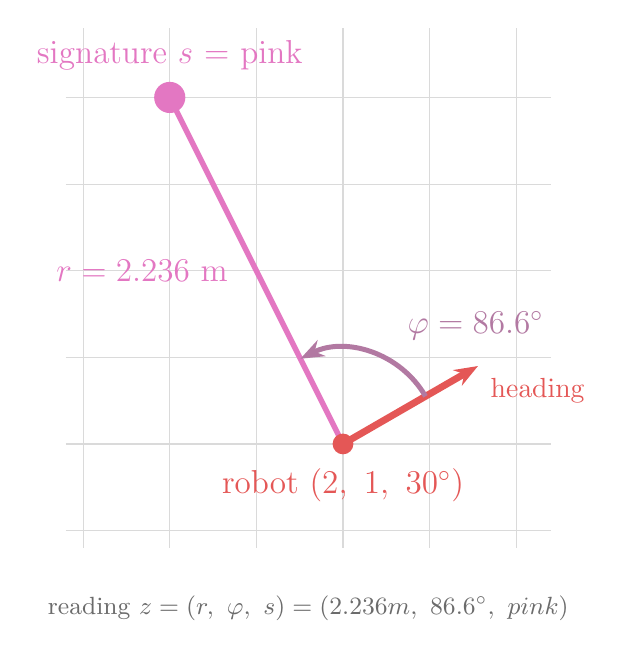
\begin{tikzpicture}[scale=2.2, every node/.append style={font=\large}]
  \definecolor{cpink}{HTML}{E377C2}
  \draw[cgrey!25, line width=0.4pt] (0.4,0.4) grid[step=0.5] (3.2,3.4);
  \coordinate (R) at (2,1); \coordinate (P) at (1,3);
  \draw[-{Stealth[length=3mm]}, cred, line width=2.5pt] (R) -- ++(30:0.9) node[below right, font=\normalsize] {heading};
  \draw[cpink, line width=2pt] (R) -- (P) node[midway, left=6pt] {$r = 2.236$ m};
  \draw[-{Stealth[length=3mm]}, cpurple, line width=1.8pt] ($(R)+(30:0.55)$) arc (30:116.6:0.55);
  \node[cpurple, anchor=south west] at ($(R)+(60:0.62)$) {$\varphi = 86.6^\circ$};
  \fill[cpink] (P) circle (0.09);
  \node[cpink, above=6pt] at (P) {signature $s$ = pink};
  \fill[cred] (R) circle (0.06); \node[cred, below] at (2,0.92) {robot $(2,\ 1,\ 30^\circ)$};
  \node[note, align=center] at (1.8,0.05) {reading $z = (r,\ \varphi,\ s) = (2.236 \text{ m},\ 86.6^\circ,\ \text{pink})$};
\end{tikzpicture}
\end{document}
